\begin{textbox}{\href{https://compneuro.neuromatch.io/tutorials/W1D5_DeepLearning/student/W1D5_Tutorial1.html}{Neural Network } }
\begin{subbox}{subbox}{Deep feed-forward networks}
\scriptsize
We can build a linear network with no hidden layers, where the stimulus prediction $y$ is a product of weights $\mathbf{W}_{out}$ and neural responses $\mathbf{r}$ with an added term $\mathbf{b}$ which is called the bias term. When you fit a linear model such as this you minimize the squared error between the predicted stimulus $y$ and the true stimulus $\tilde{y}$, this is the “loss function”. 
\begin{align}
    L &= (y - \tilde{y})^2 \\
     &= ((\mathbf{W}^{out} \mathbf{r} + \mathbf{b}) - \tilde{y})^2
\end{align}
The solution to minimizing this loss function in a linear model can be found in closed form. If we use a simple linear model for this data we are able to predict the stimulus within 2-3 degrees. 

Let’s add a hidden layer with $M$ units to this linear model, where now the output $y$ is as follows:
\begin{align}
    \mathbf{h} &= \mathbf{W}^{in} \mathbf{r} + \mathbf{b}^{in}, && [\mathbf{W}^{in}: M \times N,\, \mathbf{b}^{in}: M \times 1], \\
    y &= \mathbf{W}^{out} \mathbf{h} + \mathbf{b}^{out},  && [\mathbf{W}^{out}: 1 \times M,\, \mathbf{b}^{in}: 1 \times 1],
\end{align}

The $M$-dimensional vector $\mathbf{h}$ denotes the activations of the \textit{hidden layer} of the network. The blue components of this diagram denote the \textit{parameters} of the network, which we will later optimize with gradient descent. These include all the weights and biases $\mathbf{W}^{in}, \mathbf{b}^{in}, \mathbf{W}^{out}, \mathbf{b}^{out}$. The \textit{weights} are matrices of size (# of outputs, # of inputs) that are multiplied by the input of each layer, like the regression coefficients in linear regression.

\centering
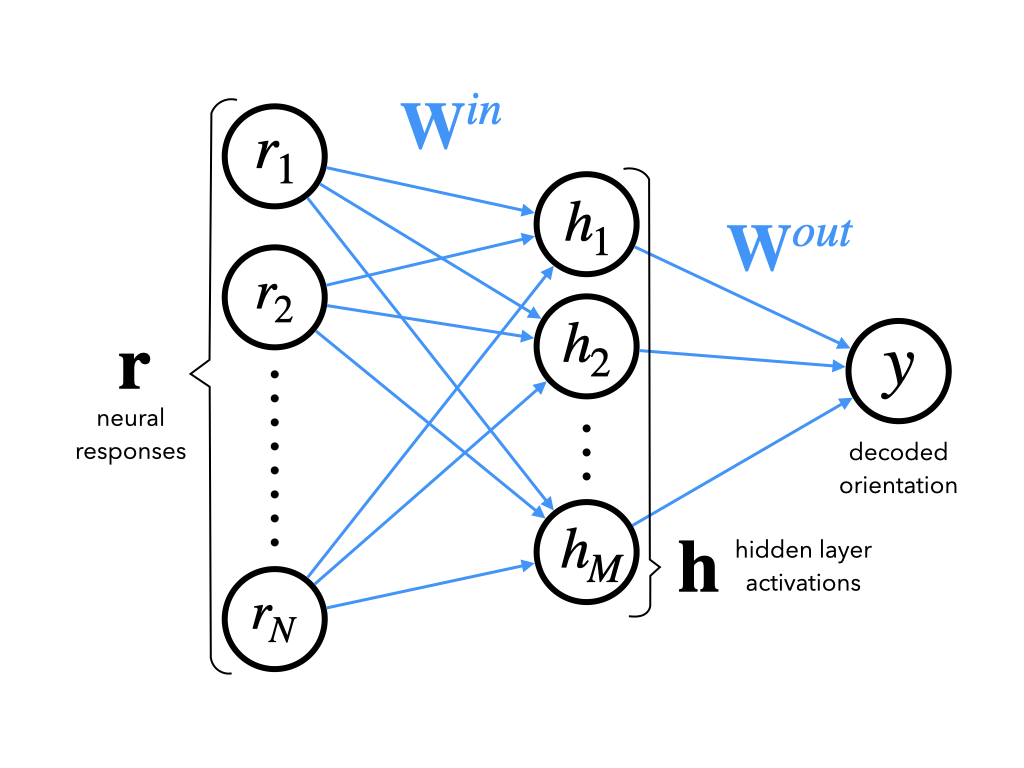
\includegraphics[scale=0.1]{Figures/DL/DLFigure1.png}
\end{subbox}


\end{textbox}
%%%%%%%%%%%%%%%%%%%%%%%%%%%%%%%%%%%%%%%%%%%%%%%%%%%%%%%
%%%%%%%%%%%%%%%%%%%%%%%%%%%%%%%%%%%%%%%%%%%%%%%%%%%%%%%
\begin{textbox}{\href{https://compneuro.neuromatch.io/tutorials/W1D5_DeepLearning/student/W1D5_Tutorial1.html}{Neural Network } }
\begin{subbox}{subbox}{Activation Functions}
\scriptsize
To extend the set of computable input/output transformations to more than just weighted sums, we'll incorporate a non-linear activation function in the hidden units. This is done by simply modifying the equation for the hidden layer activations to be
\begin{equation}
    \mathbf{h}^{(n)} = \phi(\mathbf{W}^{in} \mathbf{r}^{(n)} + \mathbf{b}^{in})
\end{equation}
where $\phi$ is referred to as the activation function. Using a non-linear activation function will ensure that the hidden layer performs a non-linear transformation of the input, which will make our network much more powerful. In practice, deep networks always use non-linear activation functions.
The most common non-linearity used is the rectified linear unit (or ReLU), which is a max(0, x) function.

\end{subbox}
\begin{subbox}{subbox}{Gradient Descent}
\scriptsize
In gradient descent we compute the gradient of the loss function with respect to each parameter (all W’s and b’s). We then update the parameters by subtracting the learning rate times the gradient. 

Let’s visualize this loss function $L$ with respect to a weight $w$. If the gradient is positive (the slope $\frac{dL}{dw}$ > 0) as in this case then we want to move in the opposite direction which is negative. So we update the $w$ accordingly in the negative direction on each iteration. Once the iterations complete the weight will ideally be at a value that minimizes the cost function.

In reality these cost functions are not convex like this one and depend on hundreds of thousands of parameters. There are tricks to help navigate this rocky cost landscape such as adding momentum or changing the optimizer but we won’t have time to get into that today. There are also ways to change the architecture of the network to improve optimization, such as including skip connections. These skip connections are used in residual networks and allow for the optimization of many layer networks.

\centering
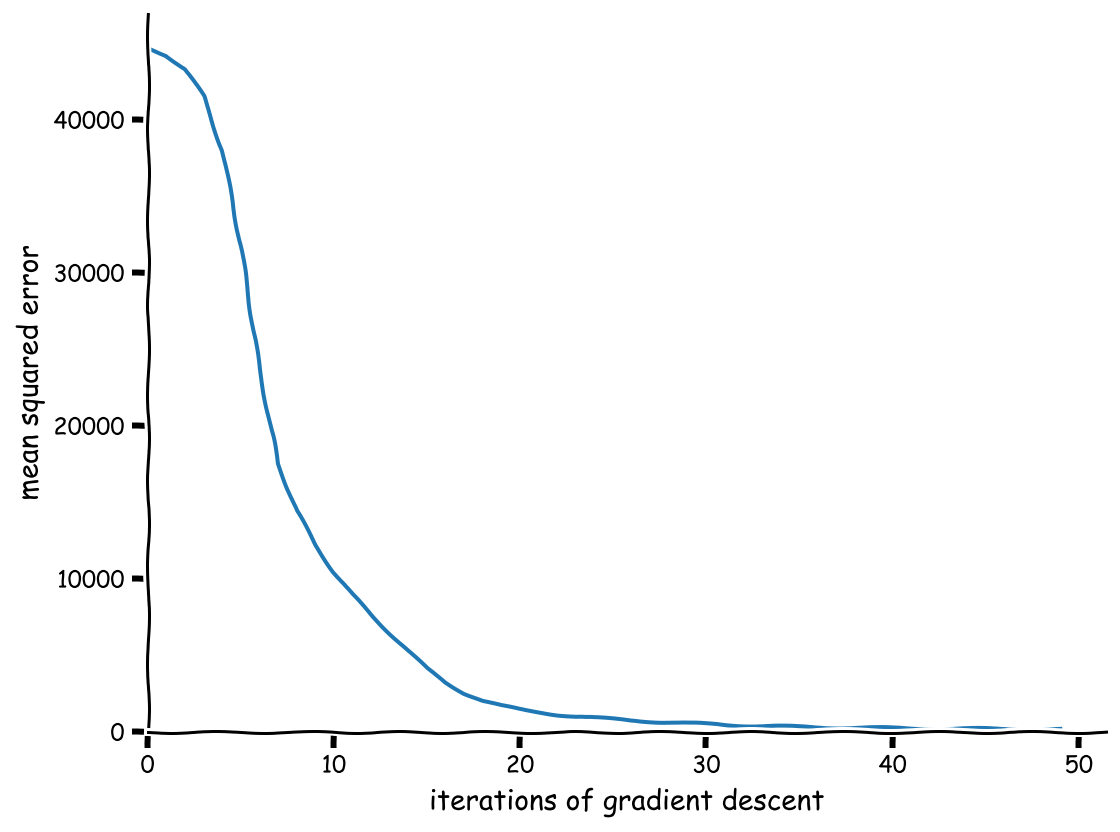
\includegraphics[scale=0.1]{Figures/DL/DLFigure2.png}
\end{subbox}

\end{textbox}
%%%%%%%%%%%%%%%%%%%%%%%%%%%%%%%%%%%%%%%%%%%%%%%%%%%%%%%
%%%%%%%%%%%%%%%%%%%%%%%%%%%%%%%%%%%%%%%%%%%%%%%%%%%%%%%
%%%%%%%%%%%%%%%%%%%%%%%%%%%%%%%%%%%%%%%%%%%%%%%%%%%%%%%
%%%%%%%%%%%%%%%%%%%%%%%%%%%%%%%%%%%%%%%%%%%%%%%%%%%%%%%
\begin{textbox}{\href{https://compneuro.neuromatch.io/tutorials/W1D5_DeepLearning/student/W1D5_Tutorial2.html}{Convolution Neural Network } }
\begin{subbox}{subbox}{Introduction to 2D convolutions}
\scriptsize
A 2D convolution is an integral of the product of a filter $f$ and an input image $I$ computed at various positions as the filter is slid across the input. The output of the convolution operation at position $(x,y)$ can be written as follows, where the filter $f$ is size $(K,K)$:
\begin{equation}
C(x,y) = \sum_{k_x=-K/2}^{K/2} \sum_{k_y=-K/2}^{K/2} f(k_x,k_y) I(x+k_x,y+k_y)
\end{equation}
This convolutional filter is often called a kernel.
\end{subbox}
%%%%%%%%%%%%%%%%%%%%%%%%%%%%%%%
\begin{subbox}{subbox}{Convolutional Layers}
\scriptsize
In a fully connected layer, each unit computes a weighted sum over all the input units. In a convolutional layer, on the other hand, each unit computes a weighted sum over only a small patch of the input, referred to as the unit's \textit{receptive field}. When the input is an image, the receptive field can be thought of as a local patch of pixels.
  
In a fully connected layer, each unit uses its own independent set of weights to compute the weighted sum. In a convolutional layer, all the units (within the same channel) share the same weights. This set of shared weights is called the convolutional filter or kernel. The result of this computation is a convolution, where each unit has computed the same weighted sum over a different part of the input. This reduces the number of parameters in the network substantially.

\centering
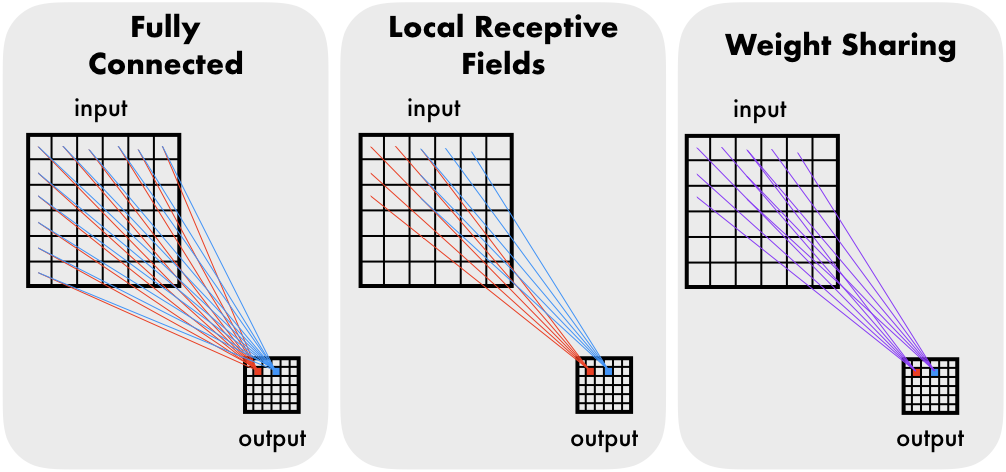
\includegraphics[scale=0.2]{Figures/DL/DLFigure3.png}
\end{subbox}
\end{textbox}
%%%%%%%%%%%%%%%%%%%%%%%%%%%%%%%%%%%%%%%%%%%%%%%%%%%%%%%
%%%%%%%%%%%%%%%%%%%%%%%%%%%%%%%%%%%%%%%%%%%%%%%%%%%%%%%
\begin{textbox}{\href{https://compneuro.neuromatch.io/tutorials/W1D5_DeepLearning/student/W1D5_Tutorial3.html}{Building and Evaluating Normative Encoding Models } }
\begin{subbox}{subbox}{Setting up Deep Network and Neural Data}
\scriptsize
We will build our normative encoding model by optimizing its parameters to solve an orientation discrimination task. 

To do this, we will use a convolutional neural network (CNN). Here, we will use a CNN that performs two-dimensional convolutions on the raw stimulus image (which is a 2D matrix of pixels), rather than one-dimensional convolutions on a categorical 1D vector representation of the stimulus. CNNs are commonly used for image processing. 

The particular CNN we will use here has two layers:
\begin{enumerate}
    \item 
a convolutional layer, which convolves the images with a set of filters
    \item a fully connected layer, which transforms the output of this convolution into a 10-dimensional representation
\end{enumerate}

Finally, a set of output weights transforms this 10-dimensional representation into a single scalar $p$, denoting the predicted probability of the input stimulus being tilted right. 

\centering
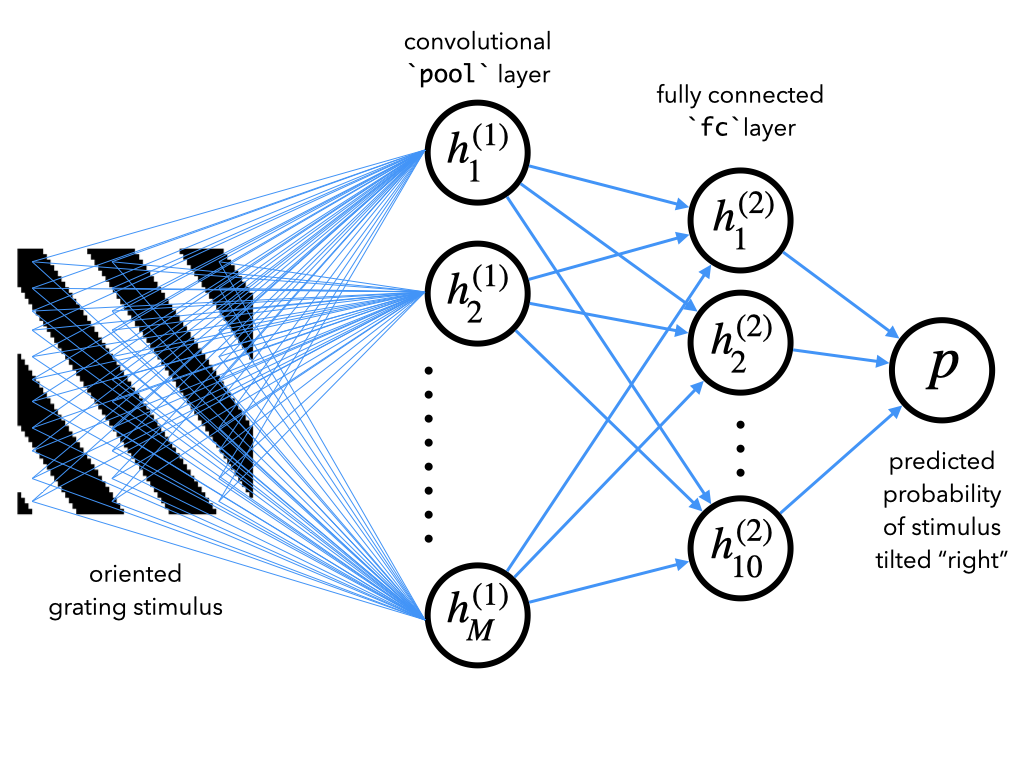
\includegraphics[scale=0.18]{Figures/DL/DLFigure4.png}

\end{subbox}
\end{textbox}
%%%%%%%%%%%%%%%%%%%%%%%%%%%%%%%%%%%%%%%%%%%%%%%%%%%%%%%
%%%%%%%%%%%%%%%%%%%%%%%%%%%%%%%%%%%%%%%%%%%%%%%%%%%%%%%
\begin{textbox}{\href{https://compneuro.neuromatch.io/tutorials/W1D5_DeepLearning/student/W1D5_Tutorial3.html}{Building and Evaluating Normative Encoding Models } }
%%%%%%%%%%%%%%%%%%%%%%%%%%%%%%%
\begin{subbox}{subbox}{Representational Dissimilarity matrix (RDM)}
\scriptsize
We noticed above some similarities and differences between the population responses in the mouse primary visual cortex and in different layers in our model. To quantify this we’ll use a technique called Representational Similarity Analysis. The idea is to look at the similarity structure between representations of different stimuli. We can say that a brain area and a model use a similar representational scheme if stimuli that are represented (dis)similarly in the brain are represented (dis)similarly in the model as well.

We begin by computing the representational dissimilarity matrix (RDM) for the mouse V1 data and each model layer. This matrix, which we'll call $\mathbf{M}$, is computed as one minus the correlation coefficients between population responses to each stimulus. We can efficiently compute this by using the $z$-scored responses. 

The $z$-scored response of all neurons $\mathbf{r}$ to stimulus $s$ is the response mean-subtracted across neurons $i$ and normalized to standard deviation 1 across neurons $i$ where $N$ is the total number of neurons:
\begin{equation}
  \mathbf{z}^{(s)} = \frac{\mathbf{r}^{(s)} - \mu^{(s)}}
  {\sigma^{(s)}}
\end{equation}
where $\mu^{(s)} = \frac{1}{N}\sum_{i=1}^N r_i^{(s)}$ and 
$\sigma^{(s)} = \sqrt{\frac{1}{N}\sum_{i=1}^N \left( r_i^{(s)} - \mu^{(s)} \right)^2}$.

Then the full matrix can be computed as:
\begin{gather}
  \mathbf{M} = 1 - \frac{1}{N} \mathbf{ZZ}^T
\end{gather}
where $\mathbf{Z}$ is the z-scored response matrix with rows $\mathbf{r}^{(s)}$ and N is the number of neurons (or units).

\end{subbox}
%%%%%%%%%%%%%%%%%%%%%%%%%%%%%%%
\begin{subbox}{subbox}{Determining Representation Similarity}
\scriptsize

To quantify how similar the representations are, we can simply correlate their dissimilarity matrices. For this, we'll again use the correlation coefficient. Note that dissimilarity matrices are symmetric ($M_{ss'} = M_{s's}$), so we should only use the off-diagonal terms on one side of the diagonal when computing this correlation to avoid overcounting. Moreover, we should leave out the diagonal terms, which are always equal to 0, so will always be perfectly correlated across any pair of RDM's.

\centering
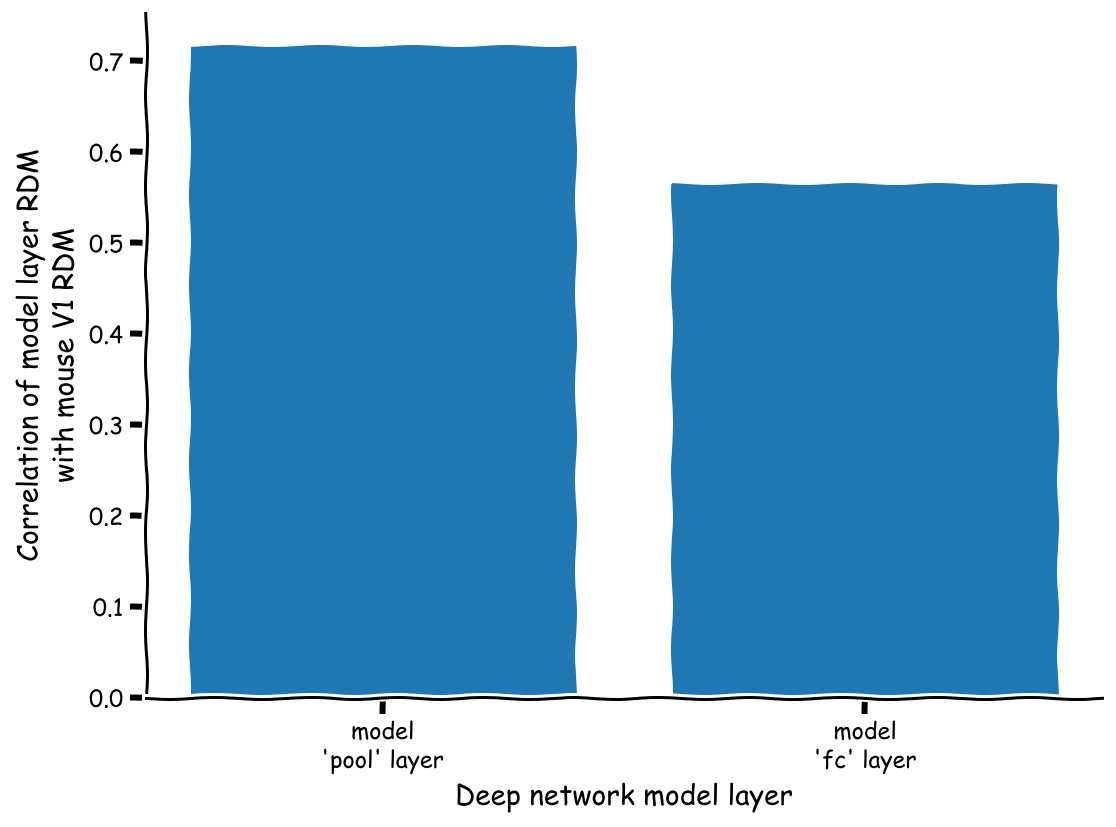
\includegraphics[scale=0.10]{Figures/DL/DLFigure5.png}

\end{subbox}
\end{textbox}

%%%%%%%%%%%%%%%%%%%%%%%%%%%%%%%%%%%%%%%%%%%%%%%%%%%%%%%
%%%%%%%%%%%%%%%%%%%%%%%%%%%%%%%%%%%%%%%%%%%%%%%%%%%%%%%
\begin{textbox}{\href{https://compneuro.neuromatch.io/tutorials/W1D5_DeepLearning/student/W1D5_Tutorial3.html}{Building and Evaluating Normative Encoding Models } }
%%%%%%%%%%%%%%%%%%%%%%%%%%%%%%%
\begin{subbox}{subbox}{Qualitative Comparisons of CNNs and Neural Activity}
\scriptsize
To visualize the representations in the data and in each of these model layers, we'll use two classic techniques from systems neuroscience:
\begin{enumerate}
    \item 
 \textbf{tuning curves}: plotting the response of single neurons (or units, in the case of the deep network) as a function of the stimulus orientation

    \item  \textbf{dimensionality reduction}: plotting full population responses to each stimulus in two dimensions via dimensionality reduction. We'll use the non-linear dimensionality reduction technique t-SNE for this. We use dimensionality reduction because there are many units and it's difficult to visualize all of them at once. We use a non-linear dimensionality reduction technique because it can capture complex relationships between stimuli.
\end{enumerate}

\end{subbox}
%%%%%%%%%%%%%%%%%%%%%%%%%%%%%%%
\begin{subbox}{subbox}{Tuning Curves}
\scriptsize
Below, we show some example tuning curves for different neurons and units in the trained CNN.

\centering
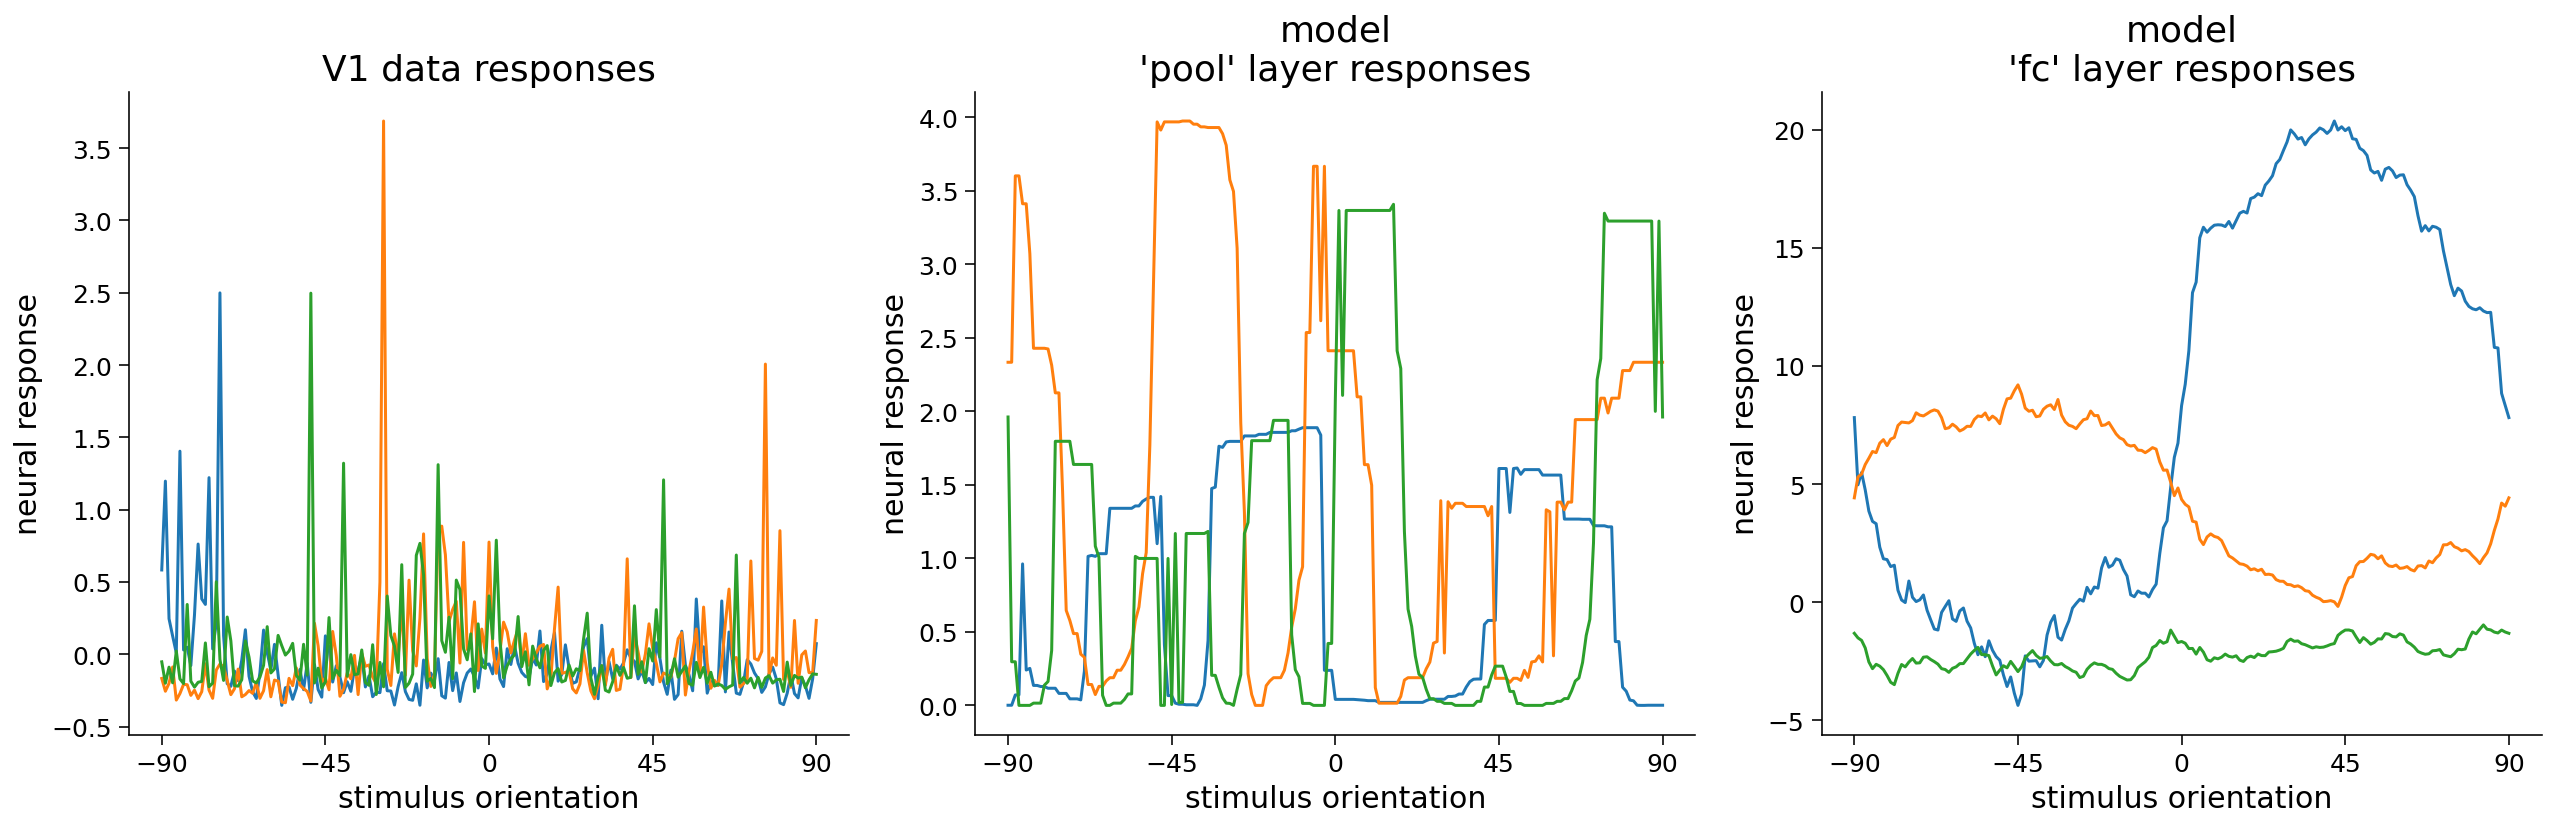
\includegraphics[scale=0.15]{Figures/DL/DLFigure6.png}

\end{subbox}
%%%%%%%%%%%%%%%%%%%%%%%%%%%%%%%
\begin{subbox}{subbox}{Dimensionality Reduction of Representations}
\scriptsize
We can visualize a dimensionality-reduced version of the internal representations of the mouse primary visual cortex or CNN internal representations in order to potentially uncover informative structure. Here, we use PCA to reduce the dimensionality to 20 dimensions, and then use tSNE to further reduce dimensionality to 2 dimensions.

\centering
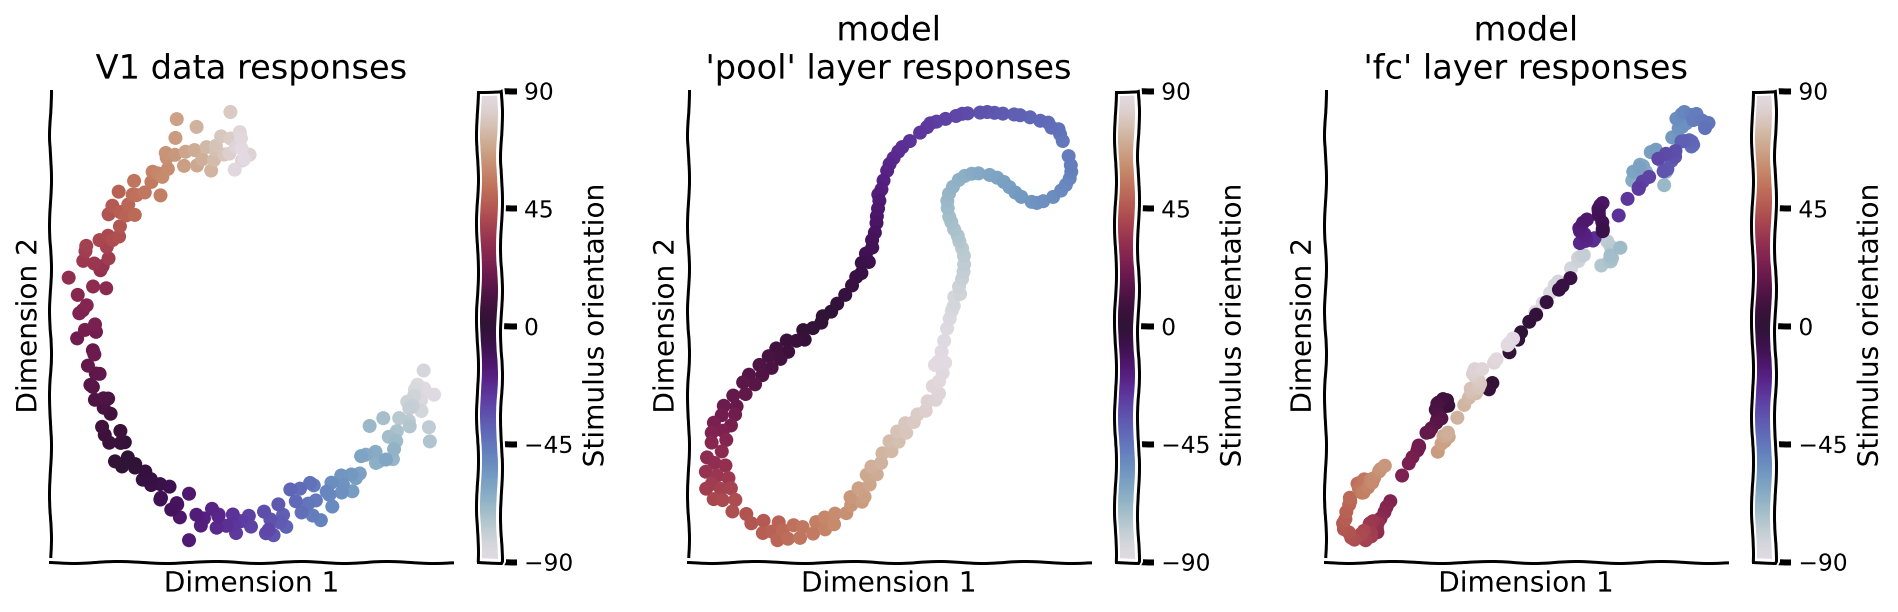
\includegraphics[scale=0.18]{Figures/DL/DLFigure7.png}

\end{subbox}
\end{textbox}